% ----------------------------------------------------------------------
%
%                            TFMTesis.tex
%
%----------------------------------------------------------------------
%
% Este fichero contiene el "documento maestro" del documento. Lo único
% que hace es configurar el entorno LaTeX e incluir los ficheros .tex
% que contienen cada sección.
%
%----------------------------------------------------------------------
%
% Los ficheros necesarios para este documento son:
%
%       TeXiS/* : ficheros de la plantilla TeXiS.
%       Cascaras/* : ficheros con las partes del documento que no
%          son capítulos ni apéndices (portada, agradecimientos, etc.)
%       Capitulos/*.tex : capítulos de la tesis
%       Apendices/*.tex: apéndices de la tesis
%       constantes.tex: constantes LaTeX
%       config.tex : configuración de la "compilación" del documento
%       guionado.tex : palabras con guiones
%
% Para la bibliografía, además, se necesitan:
%
%       *.bib : ficheros con la información de las referencias
%
% ---------------------------------------------------------------------

\documentclass[12pt,a4paper,twoside]{book}

%
% Definimos  el   comando  \compilaCapitulo,  que   luego  se  utiliza
% (opcionalmente) en config.tex. Quedaría  mejor si también se definiera
% en  ese fichero,  pero por  el modo  en el  que funciona  eso  no es
% posible. Puedes consultar la documentación de ese fichero para tener
% más  información. Definimos también  \compilaApendice, que  tiene el
% mismo  cometido, pero  que se  utiliza para  compilar  únicamente un
% apéndice.
%
%
% Si  queremos   compilar  solo   una  parte  del   documento  podemos
% especificar mediante  \includeonly{...} qué ficheros  son los únicos
% que queremos  que se incluyan.  Esto  es útil por  ejemplo para sólo
% compilar un capítulo.
%
% El problema es que todos aquellos  ficheros que NO estén en la lista
% NO   se  incluirán...  y   eso  también   afecta  a   ficheros  de
% la plantilla...
%
% Total,  que definimos  una constante  con los  ficheros  que siempre
% vamos a querer compilar  (aquellos relacionados con configuración) y
% luego definimos \compilaCapitulo.
\newcommand{\ficherosBasicosTeXiS}{%
TeXiS/TeXiS_pream,TeXiS/TeXiS_cab,TeXiS/TeXiS_bib,TeXiS/TeXiS_cover%
}
\newcommand{\ficherosBasicosTexto}{%
constantes,guionado,Cascaras/bibliografia,config%
}
\newcommand{\compilaCapitulo}[1]{%
\includeonly{\ficherosBasicosTeXiS,\ficherosBasicosTexto,Capitulos/#1}%
}

\newcommand{\compilaApendice}[1]{%
\includeonly{\ficherosBasicosTeXiS,\ficherosBasicosTexto,Apendices/#1}%
}

% #1 = tikz options (optional)
% #2 = total width (e.g. 7cm)
% #3 = height      (e.g. 0.5cm)
% #4 = wins
% #5 = draws
% #6 = losses
\newcommand{\ResultBar}[6][]{%
  \begingroup
  % compute totals & scaled lengths
  \pgfmathsetmacro{\TotalGames}{#4 + #5 + #6}%
  \pgfmathsetlengthmacro{\TotalWidth}{#2}%
  \pgfmathsetlengthmacro{\BarHeight}{#3}%
  \pgfmathsetlengthmacro{\WinWidth}{#4/\TotalGames*\TotalWidth}%
  \pgfmathsetlengthmacro{\DrawWidth}{#5/\TotalGames*\TotalWidth}%
  \pgfmathsetlengthmacro{\LossWidth}{#6/\TotalGames*\TotalWidth}%
  %
  \begin{tikzpicture}[#1]
    % coloured segments
    \fill[green!70!black] (0,0) rectangle (\WinWidth,\BarHeight);
    \fill[gray] (\WinWidth,0) rectangle (\WinWidth+\DrawWidth,\BarHeight);
    \fill[red!70!black] (\WinWidth+\DrawWidth,0)
                       rectangle (\WinWidth+\DrawWidth+\LossWidth,\BarHeight);
    % outer border
    \draw (0,0) rectangle (\TotalWidth,\BarHeight);
    % labels above each segment
    % conditional labels
    \ifnum#4>0
      \node[font=\footnotesize] at (\WinWidth/2,1.4*\BarHeight)
        {\textbf{#4} wins};
    \fi
    \ifnum#5>0
      \node[font=\footnotesize] at (\WinWidth + \DrawWidth/2,1.4*\BarHeight)
        {\textbf{#5} draws};
    \fi
    \ifnum#6>0
      \node[font=\footnotesize] at (\WinWidth+\DrawWidth + \LossWidth/2,1.4*\BarHeight)
        {\textbf{#6} losses};
    \fi
  \end{tikzpicture}%
  \endgroup
}

%- - - - - - - - - - - - - - - - - - - - - - - - - - - - - - - - - - -
%            Preámbulo del documento. Configuraciones varias
%- - - - - - - - - - - - - - - - - - - - - - - - - - - - - - - - - - -

% Define  el  tipo  de  compilación que  estamos  haciendo.   Contiene
% definiciones  de  constantes que  cambian  el  comportamiento de  la
% compilación. Debe incluirse antes del paquete TeXiS/TeXiS.sty
%---------------------------------------------------------------------
%
%                          config.tex
%
%---------------------------------------------------------------------
%
% Contiene la  definición de constantes  que determinan el modo  en el
% que se compilará el documento.
%
%---------------------------------------------------------------------
%
% En concreto, podemos  indicar si queremos "modo release",  en el que
% no  aparecerán  los  comentarios  (creados  mediante  \com{Texto}  o
% \comp{Texto}) ni los "por  hacer" (creados mediante \todo{Texto}), y
% sí aparecerán los índices. El modo "debug" (o mejor dicho en modo no
% "release" muestra los índices  (construirlos lleva tiempo y son poco
% útiles  salvo  para   la  versión  final),  pero  sí   el  resto  de
% anotaciones.
%
% Si se compila con LaTeX (no  con pdflatex) en modo Debug, también se
% muestran en una esquina de cada página las entradas (en el índice de
% palabras) que referencian  a dicha página (consulta TeXiS_pream.tex,
% en la parte referente a show).
%
% El soporte para  el índice de palabras en  TeXiS es embrionario, por
% lo  que no  asumas que  esto funcionará  correctamente.  Consulta la
% documentación al respecto en TeXiS_pream.tex.
%
%
% También  aquí configuramos  si queremos  o  no que  se incluyan  los
% acrónimos  en el  documento final  en la  versión release.  Para eso
% define (o no) la constante \acronimosEnRelease.
%
% Utilizando \compilaCapitulo{nombre}  podemos también especificar qué
% capítulo(s) queremos que se compilen. Si no se pone nada, se compila
% el documento  completo.  Si se pone, por  ejemplo, 01Introduccion se
% compilará únicamente el fichero Capitulos/01Introduccion.tex
%
% Para compilar varios  capítulos, se separan sus nombres  con comas y
% no se ponen espacios de separación.
%
% En realidad  la macro \compilaCapitulo  está definida en  el fichero
% principal tesis.tex.
%
%---------------------------------------------------------------------


% Comentar la línea si no se compila en modo release.
% TeXiS hará el resto.
% ¡¡¡Si cambias esto, haz un make clean antes de recompilar!!!
\def\release{1}


% Descomentar la linea si se quieren incluir los
% acrónimos en modo release (en modo debug
% no se incluirán nunca).
% ¡¡¡Si cambias esto, haz un make clean antes de recompilar!!!
%\def\acronimosEnRelease{1}


% Descomentar la línea para establecer el capítulo que queremos
% compilar

% \compilaCapitulo{01Introduccion}
% \compilaCapitulo{02EstructuraYGeneracion}
% \compilaCapitulo{03Edicion}
% \compilaCapitulo{04Imagenes}
% \compilaCapitulo{05Bibliografia}
% \compilaCapitulo{06Makefile}

% \compilaApendice{01AsiSeHizo}

% Variable local para emacs, para  que encuentre el fichero maestro de
% compilación y funcionen mejor algunas teclas rápidas de AucTeX
%%%
%%% Local Variables:
%%% mode: latex
%%% TeX-master: "./Tesis.tex"
%%% End:


% Paquete de la plantilla
\usepackage{TeXiS/TeXiS}

% Incluimos el fichero con comandos de constantes
%---------------------------------------------------------------------
%
%                          constantes.tex
%
%---------------------------------------------------------------------
%
% Fichero que  declara nuevos comandos LaTeX  sencillos realizados por
% comodidad en la escritura de determinadas palabras
%
%---------------------------------------------------------------------

%%%%%%%%%%%%%%%%%%%%%%%%%%%%%%%%%%%%%%%%%%%%%%%%%%%%%%%%%%%%%%%%%%%%%%
% Comando: 
%
%       \titulo
%
% Resultado: 
%
% Escribe el título del documento.
%%%%%%%%%%%%%%%%%%%%%%%%%%%%%%%%%%%%%%%%%%%%%%%%%%%%%%%%%%%%%%%%%%%%%%
\def\titulo{AlphaDeepChess: chess engine based on alpha-beta pruning}

%%%%%%%%%%%%%%%%%%%%%%%%%%%%%%%%%%%%%%%%%%%%%%%%%%%%%%%%%%%%%%%%%%%%%%
% Comando: 
%
%       \autor
%
% Resultado: 
%
% Escribe el autor del documento.
%%%%%%%%%%%%%%%%%%%%%%%%%%%%%%%%%%%%%%%%%%%%%%%%%%%%%%%%%%%%%%%%%%%%%%
\def\autor{Juan Girón Herranz y Yi Wang Qiu}

% Variable local para emacs, para  que encuentre el fichero maestro de
% compilación y funcionen mejor algunas teclas rápidas de AucTeX

%%%
%%% Local Variables:
%%% mode: latex
%%% TeX-master: "tesis.tex"
%%% End:


% Sacamos en el log de la compilación el copyright
%\typeout{Copyright Marco Antonio and Pedro Pablo Gomez Martin}

%
% "Metadatos" para el PDF
%
\ifpdf\hypersetup{%
    pdftitle = {\titulo},
    pdfsubject = {Plantilla de Tesis},
    pdfkeywords = {Plantilla, LaTeX, tesis, trabajo de
      investigación, trabajo de Master},
    pdfauthor = {\textcopyright\ \autor},
    pdfcreator = {\LaTeX\ con el paquete \flqq hyperref\frqq},
    pdfproducer = {pdfeTeX-0.\the\pdftexversion\pdftexrevision},
    }
    \pdfinfo{/CreationDate (\today)}
\fi


%- - - - - - - - - - - - - - - - - - - - - - - - - - - - - - - - - - -
%                        Documento
%- - - - - - - - - - - - - - - - - - - - - - - - - - - - - - - - - - -
\makeindex
\setlength{\parindent}{0pt} % Eliminar sangría

\begin{document}

% Incluimos el  fichero de definición de guionado  de algunas palabras
% que LaTeX no ha dividido como debería
%----------------------------------------------------------------
%
%                          guionado.tex
%
%----------------------------------------------------------------
%
% Fichero con algunas divisiones de palabras que LaTeX no
% hace correctamente si no se le da alguna ayuda.
%
%----------------------------------------------------------------

\hyphenation{
% a
abs-trac-to
abs-trac-tos
abs-trac-ta
abs-trac-tas
ac-tua-do-res
a-gra-de-ci-mien-tos
ana-li-za-dor
an-te-rio-res
an-te-rior-men-te
apa-rien-cia
a-pro-pia-do
a-pro-pia-dos
a-pro-pia-da
a-pro-pia-das
a-pro-ve-cha-mien-to
a-que-llo
a-que-llos
a-que-lla
a-que-llas
a-sig-na-tu-ra
a-sig-na-tu-ras
a-so-cia-da
a-so-cia-das
a-so-cia-do
a-so-cia-dos
au-to-ma-ti-za-do
% b
batch
bi-blio-gra-fía
bi-blio-grá-fi-cas
bien
bo-rra-dor
boo-l-ean-expr
% c
ca-be-ce-ra
call-me-thod-ins-truc-tion
cas-te-lla-no
cir-cuns-tan-cia
cir-cuns-tan-cias
co-he-ren-te
co-he-ren-tes
co-he-ren-cia
co-li-bri
co-men-ta-rio
co-mer-cia-les
co-no-ci-mien-to
cons-cien-te
con-si-de-ra-ba
con-si-de-ra-mos
con-si-de-rar-se
cons-tan-te
cons-trucción
cons-tru-ye
cons-tru-ir-se
con-tro-le
co-rrec-ta-men-te
co-rres-pon-den
co-rres-pon-dien-te
co-rres-pon-dien-tes
co-ti-dia-na
co-ti-dia-no
crean
cris-ta-li-zan
cu-rri-cu-la
cu-rri-cu-lum
cu-rri-cu-lar
cu-rri-cu-la-res
% d
de-di-ca-do
de-di-ca-dos
de-di-ca-da
de-di-ca-das
de-rro-te-ro
de-rro-te-ros
de-sa-rro-llo
de-sa-rro-llos
de-sa-rro-lla-do
de-sa-rro-lla-dos
de-sa-rro-lla-da
de-sa-rro-lla-das
de-sa-rro-lla-dor
de-sa-rro-llar
des-cri-bi-re-mos
des-crip-ción
des-crip-cio-nes
des-cri-to
des-pués
de-ta-lla-do
de-ta-lla-dos
de-ta-lla-da
de-ta-lla-das
di-a-gra-ma
di-a-gra-mas
di-se-ños
dis-po-ner
dis-po-ni-bi-li-dad
do-cu-men-ta-da
do-cu-men-to
do-cu-men-tos
% e
edi-ta-do
e-du-ca-ti-vo
e-du-ca-ti-vos
e-du-ca-ti-va
e-du-ca-ti-vas
e-la-bo-ra-do
e-la-bo-ra-dos
e-la-bo-ra-da
e-la-bo-ra-das
es-co-llo
es-co-llos
es-tu-dia-do
es-tu-dia-dos
es-tu-dia-da
es-tu-dia-das
es-tu-dian-te
e-va-lua-cio-nes
e-va-lua-do-res
exis-ten-tes
exhaus-ti-va
ex-pe-rien-cia
ex-pe-rien-cias
% f
for-ma-li-za-do
% g
ge-ne-ra-ción
ge-ne-ra-dor
ge-ne-ra-do-res
ge-ne-ran
% h
he-rra-mien-ta
he-rra-mien-tas
% i
i-dio-ma
i-dio-mas
im-pres-cin-di-ble
im-pres-cin-di-bles
in-de-xa-do
in-de-xa-dos
in-de-xa-da
in-de-xa-das
in-di-vi-dual
in-fe-ren-cia
in-fe-ren-cias
in-for-ma-ti-ca
in-gre-dien-te
in-gre-dien-tes
in-me-dia-ta-men-te
ins-ta-la-do
ins-tan-cias
% j
% k
% l
len-gua-je
li-be-ra-to-rio
li-be-ra-to-rios
li-be-ra-to-ria
li-be-ra-to-rias
li-mi-ta-do
li-te-ra-rio
li-te-ra-rios
li-te-ra-ria
li-te-ra-rias
lo-tes
% m
ma-ne-ra
ma-nual
mas-que-ra-de
ma-yor
me-mo-ria
mi-nis-te-rio
mi-nis-te-rios
mo-de-lo
mo-de-los
mo-de-la-do
mo-du-la-ri-dad
mo-vi-mien-to
% n
na-tu-ral
ni-vel
nues-tro
% o
obs-tan-te
o-rien-ta-do
o-rien-ta-dos
o-rien-ta-da
o-rien-ta-das
% p
pa-ra-le-lo
pa-ra-le-la
par-ti-cu-lar
par-ti-cu-lar-men-te
pe-da-gó-gi-ca
pe-da-gó-gi-cas
pe-da-gó-gi-co
pe-da-gó-gi-cos
pe-rio-di-ci-dad
per-so-na-je
plan-te-a-mien-to
plan-te-a-mien-tos
po-si-ción
pre-fe-ren-cia
pre-fe-ren-cias
pres-cin-di-ble
pres-cin-di-bles
pri-me-ra
pro-ble-ma
pro-ble-mas
pró-xi-mo
pu-bli-ca-cio-nes
pu-bli-ca-do
% q
% r
rá-pi-da
rá-pi-do
ra-zo-na-mien-to
ra-zo-na-mien-tos
re-a-li-zan-do
re-fe-ren-cia
re-fe-ren-cias
re-fe-ren-cia-da
re-fe-ren-cian
re-le-van-tes
re-pre-sen-ta-do
re-pre-sen-ta-dos
re-pre-sen-ta-da
re-pre-sen-ta-das
re-pre-sen-tar-lo
re-qui-si-to
re-qui-si-tos
res-pon-der
res-pon-sa-ble
% s
se-pa-ra-do
si-guien-do
si-guien-te
si-guien-tes
si-guie-ron
si-mi-lar
si-mi-la-res
si-tua-ción
% t
tem-pe-ra-ments
te-ner
trans-fe-ren-cia
trans-fe-ren-cias
% u
u-sua-rio
Unreal-Ed
% v
va-lor
va-lo-res
va-rian-te
ver-da-de-ro
ver-da-de-ros
ver-da-de-ra
ver-da-de-ras
ver-da-de-ra-men-te
ve-ri-fi-ca
% w
% x
% y
% z
}
% Variable local para emacs, para que encuentre el fichero
% maestro de compilación
%%%
%%% Local Variables:
%%% mode: latex
%%% TeX-master: "./Tesis.tex"
%%% End:


% Marcamos  el inicio  del  documento para  la  numeración de  páginas
% (usando números romanos para esta primera fase).
\frontmatter
\pagestyle{empty}

%---------------------------------------------------------------------
%
%                          configCover.tex
%
%---------------------------------------------------------------------
%
% cover.tex
% Copyright 2009 Marco Antonio Gomez-Martin, Pedro Pablo Gomez-Martin
%
% This file belongs to the TeXiS manual, a LaTeX template for writting
% Thesis and other documents. The complete last TeXiS package can
% be obtained from http://gaia.fdi.ucm.es/projects/texis/
%
% Although the TeXiS template itself is distributed under the 
% conditions of the LaTeX Project Public License
% (http://www.latex-project.org/lppl.txt), the manual content
% uses the CC-BY-SA license that stays that you are free:
%
%    - to share & to copy, distribute and transmit the work
%    - to remix and to adapt the work
%
% under the following conditions:
%
%    - Attribution: you must attribute the work in the manner
%      specified by the author or licensor (but not in any way that
%      suggests that they endorse you or your use of the work).
%    - Share Alike: if you alter, transform, or build upon this
%      work, you may distribute the resulting work only under the
%      same, similar or a compatible license.
%
% The complete license is available in
% http://creativecommons.org/licenses/by-sa/3.0/legalcode
%
%---------------------------------------------------------------------
%
% Fichero que contiene la configuración de la portada y de la 
% primera hoja del documento.
%
%---------------------------------------------------------------------


% Pueden configurarse todos los elementos del contenido de la portada
% utilizando comandos.

%%%%%%%%%%%%%%%%%%%%%%%%%%%%%%%%%%%%%%%%%%%%%%%%%%%%%%%%%%%%%%%%%%%%%%
% Título del documento:
% \tituloPortada{titulo}
% Nota:
% Si no se define se utiliza el del \titulo. Este comando permite
% cambiar el título de forma que se especifiquen dónde se quieren
% los retornos de carro cuando se utilizan fuentes grandes.
%%%%%%%%%%%%%%%%%%%%%%%%%%%%%%%%%%%%%%%%%%%%%%%%%%%%%%%%%%%%%%%%%%%%%%
\tituloPortada{%
AlphaDeepChess: motor de ajedrez basado en podas alpha-beta
}


%%%%%%%%%%%%%%%%%%%%%%%%%%%%%%%%%%%%%%%%%%%%%%%%%%%%%%%%%%%%%%%%%%%%%%
% Título del documento en inglés:
% \tituloPortadaEng{titulo}
% Nota:
% Si no se define se utiliza el del \titulo. Este comando permite
% cambiar el título de forma que se especifiquen dónde se quieren
% los retornos de carro cuando se utilizan fuentes grandes.
%%%%%%%%%%%%%%%%%%%%%%%%%%%%%%%%%%%%%%%%%%%%%%%%%%%%%%%%%%%%%%%%%%%%%%
\tituloPortadaEng{%
AlphaDeepChess: chess engine based on alpha-beta pruning
}

%%%%%%%%%%%%%%%%%%%%%%%%%%%%%%%%%%%%%%%%%%%%%%%%%%%%%%%%%%%%%%%%%%%%%%
% Autor del documento:
% \autorPortada{Nombre}
% Se utiliza en la portada y en el valor por defecto del
% primer subtítulo de la segunda portada.
%%%%%%%%%%%%%%%%%%%%%%%%%%%%%%%%%%%%%%%%%%%%%%%%%%%%%%%%%%%%%%%%%%%%%%
\autorPortada{Juan Girón Herranz \\ Yi Wang Qiu}

%%%%%%%%%%%%%%%%%%%%%%%%%%%%%%%%%%%%%%%%%%%%%%%%%%%%%%%%%%%%%%%%%%%%%%
% Fecha de publicación:
% \fechaPublicacion{Fecha}
% Puede ser vacío. Aparece en la última línea de ambas portadas
%%%%%%%%%%%%%%%%%%%%%%%%%%%%%%%%%%%%%%%%%%%%%%%%%%%%%%%%%%%%%%%%%%%%%%
% Descomentar para que ponga siempre la fecha actual
\fechaPublicacion{\today}
%\fechaPublicacion{\textcolor{red}{DIA de MES de AÑO}}

%%%%%%%%%%%%%%%%%%%%%%%%%%%%%%%%%%%%%%%%%%%%%%%%%%%%%%%%%%%%%%%%%%%%%%
% Imagen de la portada (y escala)
% \imagenPortada{Fichero}
% \escalaImagenPortada{Numero}
% Si no se especifica, se utiliza la imagen TODO.pdf
%%%%%%%%%%%%%%%%%%%%%%%%%%%%%%%%%%%%%%%%%%%%%%%%%%%%%%%%%%%%%%%%%%%%%%
% imagen en blanco y negro
%\imagenPortada{Imagenes/Vectorial/escudoUCM}
%imagen en color
\imagenPortada{Imagenes/Bitmap/escudoUCMcolor}
\escalaImagenPortada{.2}

%%%%%%%%%%%%%%%%%%%%%%%%%%%%%%%%%%%%%%%%%%%%%%%%%%%%%%%%%%%%%%%%%%%%%%
% Tipo de documento.
% \tipoDocumento{Tipo}
% Para el texto justo debajo del escudo.
% Si no se indica, se utiliza "TESIS DOCTORAL".
%%%%%%%%%%%%%%%%%%%%%%%%%%%%%%%%%%%%%%%%%%%%%%%%%%%%%%%%%%%%%%%%%%%%%%
\tipoDocumento{Trabajo de Fin de Grado}

%%%%%%%%%%%%%%%%%%%%%%%%%%%%%%%%%%%%%%%%%%%%%%%%%%%%%%%%%%%%%%%%%%%%%%
% Institución/departamento asociado al documento.
% \institucion{Nombre}
% Puede tener varias líneas. Se utiliza en las dos portadas.
% Si no se indica aparecerá vacío.
%%%%%%%%%%%%%%%%%%%%%%%%%%%%%%%%%%%%%%%%%%%%%%%%%%%%%%%%%%%%%%%%%%%%%%
\institucion{%
Grado en Ingeniería de Computadores\\[0.2em]
Facultad de Informática\\[0.2em]
Universidad Complutense de Madrid\\[0.8em]
Grado en Desarrollo de Videojuegos\\[0.2em]
Facultad de Informática\\[0.2em]
Universidad Complutense de Madrid
}

%%%%%%%%%%%%%%%%%%%%%%%%%%%%%%%%%%%%%%%%%%%%%%%%%%%%%%%%%%%%%%%%%%%%%%
% Director del trabajo.
% \directorPortada{Nombre}
% Se utiliza para el valor por defecto del segundo subtítulo, donde
% se indica quién es el director del trabajo.
% Si se fuerza un subtítulo distinto, no hace falta definirlo.
%%%%%%%%%%%%%%%%%%%%%%%%%%%%%%%%%%%%%%%%%%%%%%%%%%%%%%%%%%%%%%%%%%%%%%
\directorPortada{Ignacio Fábregas Álfaro\\Rubén Rafael Rubio Cuéllar}


%%%%%%%%%%%%%%%%%%%%%%%%%%%%%%%%%%%%%%%%%%%%%%%%%%%%%%%%%%%%%%%%%%%%%%
% Colaborador en la dirección del trabajo.
% \colaboradorPortada{Nombre}
% Se utiliza para el valor por defecto del segundo subtítulo, donde
% se indica quién es el colaborador en la dirección del trabajo.
% Si se fuerza un subtítulo distinto, no hace falta definirlo.
%%%%%%%%%%%%%%%%%%%%%%%%%%%%%%%%%%%%%%%%%%%%%%%%%%%%%%%%%%%%%%%%%%%%%%
\colaboradorPortada{\textcolor{red}{Colaborador 1\\Colaborador 2}}


%%%%%%%%%%%%%%%%%%%%%%%%%%%%%%%%%%%%%%%%%%%%%%%%%%%%%%%%%%%%%%%%%%%%%%
% Texto del primer subtítulo de la segunda portada.
% \textoPrimerSubtituloPortada{Texto}
% Para configurar el primer "texto libre" de la segunda portada.
% Si no se especifica se indica "Memoria que presenta para optar al
% título de Doctor en Informática" seguido del \autorPortada.
%%%%%%%%%%%%%%%%%%%%%%%%%%%%%%%%%%%%%%%%%%%%%%%%%%%%%%%%%%%%%%%%%%%%%%
\textoPrimerSubtituloPortada{%
\textbf{Trabajo de Fin de Grado en Ingeniería de Computadores}\\ [0.3em]
\textbf{Trabajo de Fin de Grado en Desarrollo de Videojuegos}\\ [0.3em]
}

%%%%%%%%%%%%%%%%%%%%%%%%%%%%%%%%%%%%%%%%%%%%%%%%%%%%%%%%%%%%%%%%%%%%%%
% Texto del segundo subtítulo de la segunda portada.
% \textoSegundoSubtituloPortada{Texto}
% Para configurar el segundo "texto libre" de la segunda portada.
% Si no se especifica se indica "Dirigida por el Doctor" seguido
% del \directorPortada.
%%%%%%%%%%%%%%%%%%%%%%%%%%%%%%%%%%%%%%%%%%%%%%%%%%%%%%%%%%%%%%%%%%%%%%
\textoSegundoSubtituloPortada{%
\textbf{Convocatoria: }\textit{Junio \the\year}%\\[0.2em]
%\textbf{Calificación: }\textit{\textcolor{red}{Nota}}
}

%%%%%%%%%%%%%%%%%%%%%%%%%%%%%%%%%%%%%%%%%%%%%%%%%%%%%%%%%%%%%%%%%%%%%%
% \explicacionDobleCara
% Si se utiliza, se aclara que el documento está preparado para la
% impresión a doble cara.
%%%%%%%%%%%%%%%%%%%%%%%%%%%%%%%%%%%%%%%%%%%%%%%%%%%%%%%%%%%%%%%%%%%%%%
%\explicacionDobleCara

%%%%%%%%%%%%%%%%%%%%%%%%%%%%%%%%%%%%%%%%%%%%%%%%%%%%%%%%%%%%%%%%%%%%%%
% \isbn
% Si se utiliza, aparecerá el ISBN detrás de la segunda portada.
%%%%%%%%%%%%%%%%%%%%%%%%%%%%%%%%%%%%%%%%%%%%%%%%%%%%%%%%%%%%%%%%%%%%%%
%\isbn{978-84-692-7109-4}


%%%%%%%%%%%%%%%%%%%%%%%%%%%%%%%%%%%%%%%%%%%%%%%%%%%%%%%%%%%%%%%%%%%%%%
% \copyrightInfo
% Si se utiliza, aparecerá información de los derechos de copyright
% detrás de la segunda portada.
%%%%%%%%%%%%%%%%%%%%%%%%%%%%%%%%%%%%%%%%%%%%%%%%%%%%%%%%%%%%%%%%%%%%%%
%\copyrightInfo{\autor}


%%
%% Creamos las portadas
%%
\makeCover

% Variable local para emacs, para que encuentre el fichero
% maestro de compilación
%%%
%%% Local Variables:
%%% mode: latex
%%% TeX-master: "../Tesis.tex"
%%% End:

%\include{Cascaras/autorizacion}
% +--------------------------------------------------------------------+
% | Dedication Page (Optional)
% +--------------------------------------------------------------------+

\chapter*{Dedication}

\begin{flushright}
\begin{minipage}[c]{8.5cm}
\flushright{\textit{To our younger selves, for knowing the art of chess}}
\end{minipage}
\end{flushright}
% +--------------------------------------------------------------------+
% | Acknowledgements Page (Optional)                                   |
% +--------------------------------------------------------------------+

\chapter*{Acknowledgments}

To our family members for their support and for taking us to chess tournaments to compete.












\chapter*{Abstract}

\section*{\tituloPortadaEngVal}

Chess engines have played a fundamental role in the advancement of artificial intelligence applied to the game since the mid-20th century. Pioneers such as Alan Turing and Claude Shannon established the theoretical principles that laid the foundation for this field. Building upon these foundations, the evolution of hardware and the refinement of search techniques techniques have enabled significant advancements, such as alpha-beta pruning, an optimization of the minimax algorithm that drastically reduces the number of nodes evaluated in the game tree. Today, Stockfish, the most powerful and open-source chess engine, continues to rely on alpha-beta pruning but also incorporates deep learning techniques and neural networks.

\vspace{1em}

The goal of this project is to develop a chess engine capable of competing against both other engines and human players, using alpha-beta pruning as its core. Additionally, we will analyze the impact of other classical algorithmic techniques such as transposition tables, iterative deepening, and a move generator based on magic bitboards.

\vspace{1em}

The chess engine has finally been uploaded to the Lichess.org platform, where AlphaDeepChess achieved an ELO rating of 1900 while running on a Raspberry Pi 5 equipped with a 2TB transposition table.

\section*{Keywords}

\noindent chess, chess engine, artificial intelligence, alpha-beta pruning, iterative deepening, quiescence search, move ordering, transposition table, zobrist hashing, pext instruction, magic bitboards

\begin{otherlanguage}{english} % para que aparezca ingles y luego espanol
  \chapter*{Resumen}

\section*{\tituloPortadaVal}

Los motores de ajedrez han desempeñado un papel fundamental en el avance de la inteligencia artificial aplicada al juego desde mediados del siglo XX. Pioneros como Alan Turing y Claude Shannon establecieron los principios teóricos que sentaron las bases de este campo. Sobre estos cimientos, la evolución del hardware y el perfeccionamiento de técnicas de búsqueda permitieron importantes avances, como la poda alfa-beta, una optimización del algoritmo minimax que reduce drásticamente el número de nodos evaluados en el árbol de juego. Hoy en día, Stockfish, el motor de ajedrez más potente y de código abierto, sigue basándose en técnicas algorítmicas clásicas, pero también incorpora de deep learning y redes neuronales.

\vspace{1em}

El objetivo de este proyecto es desarrollar un motor de ajedrez capaz de competir tanto contra otros motores como contra jugadores humanos, utilizando la poda alfa-beta como núcleo del algoritmo. Además, se analizará el impacto de otras técnicas algorítmicas clásicas, como las tablas de transposición, la búsqueda en profundidad iterativa y un generador de movimientos basado en bitboards mágicos.

\vspace{1em}

Finalmente, el motor de ajedrez ha sido subido a la plataforma Lichess.org, donde AlphaDeepChess ha alcanzado una puntuación ELO de 1900, ejecutándose en una Raspberry Pi 5 con una tabla de transposiciones de 2TB.

\section*{Palabras clave}
   
\noindent ajedrez, motor de ajedrez, inteligencia artificial, poda alfa-beta, búsqueda en profundidad iterativa, búsqueda quiescente, ordenación de movimientos, tabla de transposiciones, zobrist hashing, instrucción pext, bitboards mágicos 
   



% Si el trabajo se escribe en inglés, comentar esta línea y descomentar
% otra igual que hay justo antes de \end{document}
\end{otherlanguage}

\ifx\generatoc\undefined
\else
%---------------------------------------------------------------------
%
%                          TeXiS_toc.tex
%
%---------------------------------------------------------------------
%
% TeXiS_toc.tex
% Copyright 2009 Marco Antonio Gomez-Martin, Pedro Pablo Gomez-Martin
%
% This file belongs to TeXiS, a LaTeX template for writting
% Thesis and other documents. The complete last TeXiS package can
% be obtained from http://gaia.fdi.ucm.es/projects/texis/
%
% This work may be distributed and/or modified under the
% conditions of the LaTeX Project Public License, either version 1.3
% of this license or (at your option) any later version.
% The latest version of this license is in
%   http://www.latex-project.org/lppl.txt
% and version 1.3 or later is part of all distributions of LaTeX
% version 2005/12/01 or later.
%
% This work has the LPPL maintenance status `maintained'.
% 
% The Current Maintainers of this work are Marco Antonio Gomez-Martin
% and Pedro Pablo Gomez-Martin
%
%---------------------------------------------------------------------
%
% Contiene  los  comandos  para  generar los  índices  del  documento,
% entendiendo por índices las tablas de contenidos.
%
% Genera  el  índice normal  ("tabla  de  contenidos"),  el índice  de
% figuras y el de tablas. También  crea "marcadores" en el caso de que
% se esté compilando con pdflatex para que aparezcan en el PDF.
%
%---------------------------------------------------------------------


% Primero un poquito de configuración...


% Pedimos que inserte todos los epígrafes hasta el nivel \subsection en
% la tabla de contenidos.
\setcounter{tocdepth}{2} 

% Le  pedimos  que nos  numere  todos  los  epígrafes hasta  el  nivel
% \subsubsection en el cuerpo del documento.
\setcounter{secnumdepth}{3} 


% Creamos los diferentes índices.

% Lo primero un  poco de trabajo en los marcadores  del PDF. No quiero
% que  salga una  entrada  por cada  índice  a nivel  0...  si no  que
% aparezca un marcador "Índices", que  tenga dentro los otros tipos de
% índices.  Total, que creamos el marcador "Índices".
% Antes de  la creación  de los índices,  se añaden los  marcadores de
% nivel 1.

\ifpdf
   \pdfbookmark{Índices}{indices}
\fi

% Tabla de contenidos.
%
% La  inclusión  de '\tableofcontents'  significa  que  en la  primera
% pasada  de  LaTeX  se  crea   un  fichero  con  extensión  .toc  con
% información sobre la tabla de contenidos (es conceptualmente similar
% al  .bbl de  BibTeX, creo).  En la  segunda ejecución  de  LaTeX ese
% documento se utiliza para  generar la verdadera página de contenidos
% usando la  información sobre los  capítulos y demás guardadas  en el
% .toc
\ifpdf
   \pdfbookmark[1]{Tabla de Contenidos}{tabla de contenidos}
\fi

\cabeceraEspecial{\'Indice}

\tableofcontents

\newpage 

% Índice de figuras
%
% La idea es semejante que para  el .toc del índice, pero ahora se usa
% extensión .lof (List Of Figures) con la información de las figuras.

\ifpdf
   \pdfbookmark[1]{Índice de figuras}{indice de figuras}
\fi

\cabeceraEspecial{\'Indice de figuras}

\listoffigures

\newpage

% Índice de tablas
% Como antes, pero ahora .lot (List Of Tables)

\ifpdf
   \pdfbookmark[1]{Índice de tablas}{indice de tablas}
\fi

\cabeceraEspecial{\'Indice de tablas}

\listoftables

\newpage

% Variable local para emacs, para  que encuentre el fichero maestro de
% compilación y funcionen mejor algunas teclas rápidas de AucTeX

%%%
%%% Local Variables:
%%% mode: latex
%%% TeX-master: "../Tesis.tex"
%%% End:

\fi

% Marcamos el  comienzo de  los capítulos (para  la numeración  de las
% páginas) y ponemos la cabecera normal
\mainmatter

\pagestyle{fancy}
\restauraCabecera

\chapter{Introduction}
\label{cap:introduction}

\chapterquote{The most powerful weapon in chess is to have the next move}{David Bronstein}

Chess, one of the oldest and most strategic games in human history, has long been a domain for both intellectual competition and computational research. The pursuit of creating a machine that could compete with the best human players, chess Grandmasters (GM), was present. It was only a matter of time before computation surpassed human computational capabilities.

In 1997, the chess engine Deep Blue made history by defeating the world champion at the time, Garry Kasparov, marking the first time a computer had defeated a reigning world champion in a six-game match under standard chess tournament time controls\footnote{\url{https://en.wikipedia.org/wiki/Deep_Blue_(chess_computer)}}.

Since then, the development of chess engines has advanced rapidly, moving from rule-based systems to AI-driven models. However, classical search algorithms, such as alpha-beta pruning, continue to be fundamental to understanding the basics of efficient search and evaluation of game trees.

%\section{Motivation}

\section{Objetives}

\begin{itemize}
    \item Develop a functional chess engine using alpha-beta pruning as the core search algorithm.
    \item Optimize search efficiency by implementing move ordering, quiescence search, and iterative deepening to improve pruning effectiveness.
    \item Implement transposition tables using Zobrist hashing to store and retrieve previously evaluated board positions efficiently.
    \item Ensure modularity and efficiency so that the engine can be tested, improved, and integrated into chess-playing applications.
    \item Compare performance metrics against other classical engines to evaluate the impact of implemented optimizations.
\end{itemize}

\section{Work plan}

\begin{enumerate}
    \item Research phase and basic implementation: understand the fundamentals of alpha-beta pruning with minimax and position evaluation. Familiarize with the UCI (Universal Chess Interface) and implement the move generator with its specific exceptions and rules.
    \item Optimization: improve search efficiency using transposition tables and Zobrist hashing.
    \item Comparation: use Stockfish to compare efficiency generating tournaments between chess engines and a profiler to detect possible bottlenecks.
\end{enumerate}

%\section{Explicaciones adicionales sobre el uso de esta plantilla}
%Si quieres cambiar el \textbf{estilo del título} de los capítulos del documento, edita el fichero \verb|TeXiS\TeXiS_pream.tex| y comenta la línea \verb|\usepackage[Lenny]{fncychap}| para dejar el estilo básico de \LaTeX.

%Si no te gusta que no haya \textbf{espacios entre párrafos} y quieres dejar un pequeño espacio en blanco, no metas saltos de línea (\verb|\\|) al final de los párrafos. En su lugar, busca el comando  \verb|\setlength{\parskip}{0.2ex}| en \verb|TeXiS\TeXiS_pream.tex| y aumenta el valor de $0.2ex$ a, por ejemplo, $1ex$.

%TFGTeXiS se ha elaborado a partir de la plantilla de TeXiS\footnote{\url{http://gaia.fdi.ucm.es/research/texis/}}, creada por Marco Antonio y Pedro Pablo Gómez Martín para escribir su tesis doctoral. Para explicaciones más extensas y detalladas sobre cómo usar esta plantilla, recomendamos la lectura del documento \texttt{TeXiS-Manual-1.0.pdf} que acompaña a esta plantilla.

%El siguiente texto se genera con el comando \verb|\lipsum[2-20]| que viene a continuación en el fichero .tex. El único propósito es mostrar el aspecto de las páginas usando esta plantilla. Quita este comando y, si quieres, comenta o elimina el paquete \textit{lipsum} al final de \verb|TeXiS\TeXiS_pream.tex|

%\subsection{Texto de prueba}


%\lipsum[2-20]
\chapter{Estado de la Cuestión}
\label{cap:estadoDeLaCuestion}

En el estado de la cuestión es donde aparecen gran parte de las referencias bibliográficas del trabajo. Una de las formas más cómodas de gestionar la bibliografía en {\LaTeX} es utilizando \textbf{bibtex}. Las entradas bibliográficas deben estar en un fichero con extensión \textit{.bib} (con esta plantilla se proporciona el fichero biblio.bib, donde están las entradas referenciadas más abajo). Cada entrada bibliográfica tiene una clave que permite referenciarla desde cualquier parte del texto con los siguiente comandos:

\begin{itemize}
\item Referencia bibliografica con cite: \cite{ldesc2e}
\item Referencia bibliográfica con citep: \citep{notsoshort}
\item Referencia bibliográfica con citet: \citet{latexAPrimer}
\end{itemize}

Es posible citar más de una fuente, como por ejemplo \citep{latexCompanion,LaTeXLamport,texKnuth}

Después, \LaTeX se ocupa de rellenar la sección de bibliografía con las entradas \textbf{que hayan sido citadas} (es decir, no con todas las entradas que hay en el .bib, sino sólo con aquellas que se hayan citado en alguna parte del texto).

Bibtex es un programa separado de latex, pdflatex o cualquier otra cosa que se use para compilar los .tex, de manera que para que se rellene correctamente la sección de bibliografía es necesario compilar primero el trabajo (a veces es necesario compilarlo dos veces), compilar después con bibtex, y volver a compilar otra vez el trabajo (de nuevo, puede ser necesario compilarlo dos veces). 

\chapter{Work description}
\label{cap:descripcionTrabajo}

\section{Modules}
\label{sec:modules}

\subsection{Board}

\subsection{Move generator}

\subsection{Move ordering}

\subsection{Evaluation}

\subsection{Search}

\section{Code implementation}

\subsection{Data representation}

Use of uint64\_t as bitboards to store the board information and other code structures and classes justifying why is efficient.

\subsection{Initialized memory}

Some tables are memory initialized instead of computed, explain it.

\section{Additional tools and work}

\subsection{Board visualizer using Python}

\subsection{Comparation using Cutechess and Stockfish engine}

\subsection{Profiling}

\chapter{Improvement Techniques}\label{cap:ImprovementTechniques}

This chapter documents the implementation of the following techniques used to improve the chess engine:

\begin{itemize}[itemsep=1pt]
    \item Transposition tables with zobrist hashing.
    \item Move generator with magic bitboards and PEXT instructions.
    \item Evaluation with king safety and piece mobility parameters.
    \item Multithread search.
    \item Search with Late move Reductions.
\end{itemize}
\section{Transposition Table}\label{sec:tt}

\noindent As discused in the previous chapter (see~\cref{sec:iterativeDeepening}), the basic implementation of the chess engine generates a large amount of redundant calculations due to the iterative deepening approach and also the concept of transpositions: situations in which the same board position is reached through different sequences of moves in the game tree.
\noindent~\cref{fig:transposition_example} illustrates a position that can arise through multiple move orders. Where the white king could go to the g3 square from multiple paths.

\begin{figure}
    \centering
    \begin{minipage}{0.6\textwidth}
        \centering
        \newchessgame
        \chessboard[
            showmover=false,
            setfen=8/2k5/3p4/p2P1p2/P2P1P2/8/8/2K5 w - - 0 1,
            pgfstyle=straightmove, color=blue,
            markmoves={c1-e3,e3-g3,c1-g1,g1-g3},
            arrow=to
        ]
    \end{minipage}
    \caption{Lasker-Reichhelm Position, transposition example}\label{fig:transposition_example}
\end{figure}

\vspace{1em}

\noindent Taking advantage of dynamic programming, we create a look-up table of chess positions and its evaluation. So if we encounter the same position again, the evaluation is already precalculated. However, we ask ourselves the following question: how much space does the look-up table take up if there are an astronomical amount of chess positions? What we can do is assign a hash to each position and make the table index the last bits of the hash. The larger the table, the less likely access collisions will be. We also want a hash that is fast to calculate and has collision-reducing properties.
~\cite{TranspositionTable}

\vspace{1em}

\noindent \parbox{\textwidth}{The complete implementation can be found in\\\texttt{include\textbackslash{}utilities\textbackslash{}transposition\_table.hpp}.}

\subsection{Zobrist Hashing}

Zobrist Hashing is a technique to transform a board position of arbitrary size into a number of a set length, with an equal distribution over all possible numbers invented by Albert Zobrist~\cite{ZobristHashing}.

\vspace{1em}

\noindent To generate a 64-bit hash for a position, the following steps are followed:

\begin{enumerate}
  \item Pseudorandom 64-bit numbers are generated for each possible feature of a position:
  \begin{enumerate}
    \item One number for each piece type on each square — 12 pieces x 64 squares = 768 numbers.
    \item One number to indicate the side to move is black.
    \item Four numbers to represent castling rights (kingside and queenside for both white and black).
    \item Eight numbers to represent the file of an available \textit{en passant} square.
  \end{enumerate}
  \item The final hash is computed by XOR-ing together all the random numbers corresponding to the features present in the current position.
\end{enumerate}

\noindent These random values ensure that even slightly different positions produce very different hash values. This greatly reduces the chance of collisions.

\vspace{1em}

\noindent The XOR operation is used not only because it is computationally inexpensive, but also because it is reversible. This means that when a move is made or undone, we can update the hash incrementally by applying XOR only to the affected squares, without needing to recompute the entire hash.

\vspace{1em}

\noindent The position shown in~\cref{fig:zobristExamplePosition} illustrates an example of how the Zobrist hash is computed.  
The hash value is calculated by XORing the random values associated with each element of the position.  
Since the side to move is White, we do not XOR the value associated with Black to move.  
The resulting hash is computed as follows:

\[
111 \oplus 69 \oplus 909 \oplus 10 \oplus 67 \oplus 12 \oplus 555 \oplus 3 = 458
\]

\noindent Where $\oplus$ denotes $XOR$.

\begin{figure}
    \centering
    \begin{minipage}[t]{0.4\textwidth}
        \centering
        \newchessgame
        \chessboard[
            showmover=true,
            setfen=7r/8/k7/1pP5/8/4Q3/1P6/1K6 w - b6 0 1,
            markstyle=circle,
            color=blue, markfields={b6},
            pgfstyle=straightmove, color=red,
            markmoves={b7-b5},
            arrow=to
        ]
        \caption*{Side to move is white. The last move was a pawn advancing from b7 to b5, making \text{en passant} available on the b6 square.}
    \end{minipage}
    \hspace{1cm}
    \begin{minipage}[t]{0.4\textwidth}
        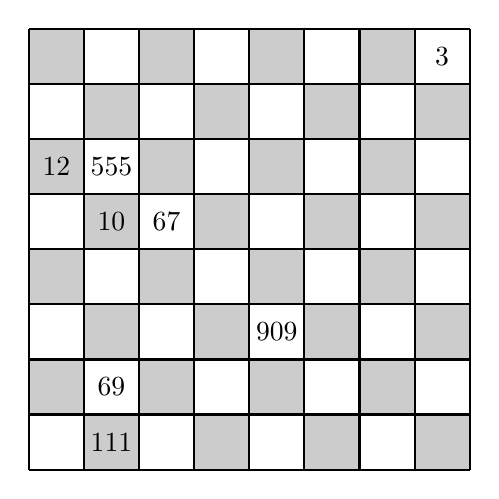
\begin{tikzpicture}[scale=0.7]

            \foreach \x in {0,1,...,7} {
                \foreach \y in {0,1,...,7} {
                    \pgfmathparse{mod(\x+\y,2) ? "black!20" : "white"}
                    \edef\col{\pgfmathresult}
                    \fill[\col] (\x,\y) rectangle (\x+1,\y+1);
                }
            }

            \node at (1.5,0.5) {111}; \node at (1.5,1.5) {69}; \node at (4.5,2.5) {909}; \node at (1.5,4.5) {10};
            \node at (2.5,4.5) {67}; \node at (0.5,5.5) {12}; \node at (1.5,5.5) {555}; \node at (7.5,7.5) {3};

            \draw[thick] (0,0) grid (8,8);
        \end{tikzpicture}
        \vspace{1.5em}
        \caption*{Random values corresponding to each piece and the en passant square. The value for Black to move is 62319.}
    \end{minipage}
    \caption{Zobrist hash calculation example.}\label{fig:zobristExamplePosition}
\end{figure}

\subsection{Table Entry}

Each entry in the transposition table stores the following information:

\begin{enumerate}
  \item \textit{Zobrist Hash}: The full 64-bit hash of the position. This is used to verify that the entry corresponds to the current position and to detect possible index collisions in the table.
  \item \textit{Evaluation}: The numerical evaluation of the position, as computed by the evaluation function.
  \item \textit{Depth}: The depth at which the evaluation was calculated. A deeper search could potentially yield a more accurate evaluation, so this value helps determine whether a new evaluation should overwrite the existing one.
  \item \textit{Node Type}: Indicates the type of node stored:
  \begin{enumerate}
    \item \textit{EXACT} the evaluation is precise for this position.
    \item \textit{UPPERBOUND} the evaluation is an upper bound, typically resulting from an alpha cutoff.
    \item \textit{LOWERBOUND} the evaluation is a lower bound, typically resulting from a beta cutoff.
    \item \textit{FAILED} entry is empty or with invalid information.
  \end{enumerate}
\end{enumerate}

\subsection{Collisions}

As discussed earlier, index collisions in the transposition table are handled by verifying the full Zobrist hash stored in the entry. However, it is still theoretically possible for a full hash collision to occur, that is two different positions producing the same hash.

\vspace{1em}

\noindent This scenario is extremely rare. With 64-bit hashes, there are $2^{64}$ possible unique values, which is more than sufficient for practical purposes. In the unlikely event of a true hash collision, it could result in an incorrect evaluation being reused for a different position.

\section{Move generator with Magic Bitboards and PEXT instructions}

To identify potential performance bottlenecks, we performed profiling on the engine, as shown in~\cref{fig:profiling}.

\vspace{1em}

\begin{figure}
    \centering
    \includegraphics[width=1.0\textwidth]{Imagenes/basic_move_generator_profiling.png}
    \caption{Profiling results.}\label{fig:profiling}
\end{figure}

\noindent The profiling results indicate that the majority of the total execution time is spent in the legal move generation function. Therefore, optimizing this component is expected to yield significant performance improvements.

\subsection{Magic bitboards}

We can create a look up table of all the rook and bishop moves for each square on the board and for each combination of pieces that blocks the path of the slider piece (blockers  bitboard). Basically we need a hash table to store rook and bishop moves indexed by square and bitboard of blockers. The problem is that this table could be very big~\cite{MagicBitboards}.

\vspace{1em}

\noindent Magic bitboards technique used to reduce the size of the look up table. We cut off unnecesary information in the blockers bitboard, excluding the board borders and the squares outside its attack pattern.

\vspace{1em}

\noindent A \textbf{magic number} is a multiplier to the bitboard of blockers with the following properties:

\begin{itemize}[itemsep=1pt]
  \item Preserves relevant blocker information: 
  The nearest blockers along a piece's movement direction are preserved. 
  \textit{Example:} Consider a rook with two pawns in its path:
  \begin{center}
    Rook $\rightarrow \rightarrow \rightarrow$ [Pawn1][Pawn2]
  \end{center}
  In this case, only `Pawn1` blocks the rook's movement, while `Pawn2` is irrelevant.
  \item Compresses the blocker bitboard, pushing the important bits near the most significant bit.
  \item The final multiplication must produce a unique index for each possible blocker configuration. The way to ensure the uniqueness is by brute force testing.
\end{itemize}

\noindent As illustrated in~\ref{fig:magics_position}, we aim to compute the legal moves of the white rook in the given position. In practice, the only pieces that truly block the rook's path are those marked with a red circle.

\vspace{1em}

\begin{figure}
    \centering
    \begin{minipage}{0.6\textwidth}
        \centering
        \newchessgame
        \chessboard[
            showmover=false,
            setfen=n1bk3r/3p4/1p1p2p1/8/3R1p2/8/3p4/7n w - - 0 1,
            markstyle=circle,
            color=red, markfields={d6,f4,d2},
            color=green, markfields={c4,b4,a4,e4,d5,d3}
        ]
    \end{minipage}
    \caption{Initial chess position with white rook and blockers}\label{fig:magics_position}
\end{figure}

\subsection*{Magic number generation}

\noindent
Magic numbers are generated through a trial and error process. For each square on the board,random numbers are tested until one produces a unique index for every possible blocker configuration~\cite{MagicBitboards}. Over the years, the chess programming community has discovered better magic numbers. In this project, we use magics sourced from the Chess Programming YouTube channel~\cite{MagicsSource}.


\subsection*{Index calculation}

\noindent First, we mask out all pieces outside the rook's attack pattern or on the board borders, as shown in~\ref{fig:magic_preprocessing}.

\vspace{1em}

\begin{figure}
    \centering
    \begin{minipage}[c]{0.4\textwidth}
        \centering
        \includegraphics[width=\textwidth]{Imagenes/magics_blockers.png}
        \caption{Original blockers bitboard}
    \end{minipage}
    \hfill
    \begin{minipage}[c]{0.1\textwidth}
        \centering
        \small$\to$
    \end{minipage}
    \hfill
    \begin{minipage}[c]{0.4\textwidth}
        \centering
        \includegraphics[width=\textwidth]{Imagenes/magics_processed_blockers.png}
        \caption{Masked blockers bitboard}
    \end{minipage}
    \caption{Pre-processing of the blockers bitboard}\label{fig:magic_preprocessing}
\end{figure}

\noindent As illustrated in~\ref{fig:magic_multiplication}, the masked blockers bitboard is then multiplied by the magic number. The result retains only the three relevant pawns that obstruct the rook's movement, pushing them toward the most significant bits.

\vspace{1em}

\begin{figure}
    \centering
    \begin{minipage}[c]{0.4\textwidth}
        \centering
        \includegraphics[width=\textwidth]{Imagenes/magics_processed_blockers.png}
        \caption{Masked blockers bitboard}
    \end{minipage}
    \hfill
    \begin{minipage}[c]{0.1\textwidth}
        \centering
        \Huge$\times$ \\[0.5em]
        \small Magic number \\[0.5em]
        \Huge$=$
    \end{minipage}
    \hfill
    \begin{minipage}[c]{0.4\textwidth}
        \centering
        \includegraphics[width=\textwidth]{Imagenes/magics_multiplied_blockers.png}
        \caption{Multiplied blockers bitboard}
    \end{minipage}
    \caption{Multiplication by magic number to produce an index}\label{fig:magic_multiplication}
\end{figure}

\noindent Next, we compress the index toward the least significant bits by shifting right by \(\,64-\)\texttt{relevant\_squares}. The number of relevant squares varies per board square; ~\ref{fig:rook_relevant_squares} shows this for the rook:

\vspace{1em}

\begin{figure}
    \centering
    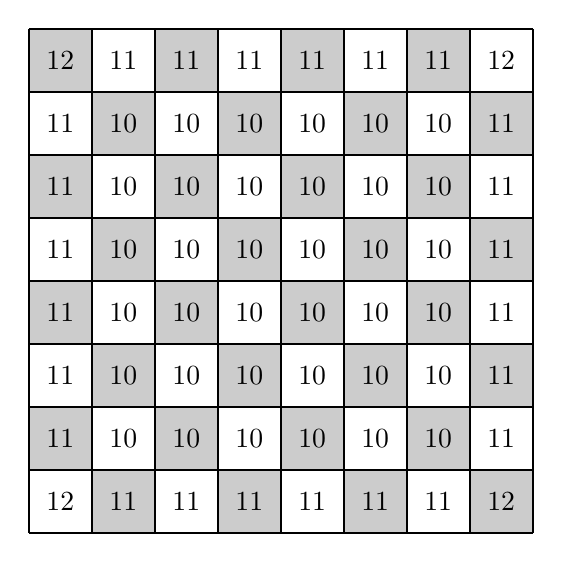
\begin{tikzpicture}[scale=0.8]
        % Draw the chessboard
        \foreach \x in {0,1,...,7} {
            \foreach \y in {0,1,...,7} {
                \pgfmathparse{mod(\x+\y,2) ? "black!20" : "white"}
                \edef\col{\pgfmathresult}
                \fill[\col] (\x,\y) rectangle (\x+1,\y+1);
            }
        }

        % Add the values to the squares
        \node at (0.5,7.5) {12}; \node at (1.5,7.5) {11}; \node at (2.5,7.5) {11}; \node at (3.5,7.5) {11};
        \node at (4.5,7.5) {11}; \node at (5.5,7.5) {11}; \node at (6.5,7.5) {11}; \node at (7.5,7.5) {12};

        \node at (0.5,6.5) {11}; \node at (1.5,6.5) {10}; \node at (2.5,6.5) {10}; \node at (3.5,6.5) {10};
        \node at (4.5,6.5) {10}; \node at (5.5,6.5) {10}; \node at (6.5,6.5) {10}; \node at (7.5,6.5) {11};

        \node at (0.5,5.5) {11}; \node at (1.5,5.5) {10}; \node at (2.5,5.5) {10}; \node at (3.5,5.5) {10};
        \node at (4.5,5.5) {10}; \node at (5.5,5.5) {10}; \node at (6.5,5.5) {10}; \node at (7.5,5.5) {11};

        \node at (0.5,4.5) {11}; \node at (1.5,4.5) {10}; \node at (2.5,4.5) {10}; \node at (3.5,4.5) {10};
        \node at (4.5,4.5) {10}; \node at (5.5,4.5) {10}; \node at (6.5,4.5) {10}; \node at (7.5,4.5) {11};

        \node at (0.5,3.5) {11}; \node at (1.5,3.5) {10}; \node at (2.5,3.5) {10}; \node at (3.5,3.5) {10};
        \node at (4.5,3.5) {10}; \node at (5.5,3.5) {10}; \node at (6.5,3.5) {10}; \node at (7.5,3.5) {11};

        \node at (0.5,2.5) {11}; \node at (1.5,2.5) {10}; \node at (2.5,2.5) {10}; \node at (3.5,2.5) {10};
        \node at (4.5,2.5) {10}; \node at (5.5,2.5) {10}; \node at (6.5,2.5) {10}; \node at (7.5,2.5) {11};

        \node at (0.5,1.5) {11}; \node at (1.5,1.5) {10}; \node at (2.5,1.5) {10}; \node at (3.5,1.5) {10};
        \node at (4.5,1.5) {10}; \node at (5.5,1.5) {10}; \node at (6.5,1.5) {10}; \node at (7.5,1.5) {11};

        \node at (0.5,0.5) {12}; \node at (1.5,0.5) {11}; \node at (2.5,0.5) {11}; \node at (3.5,0.5) {11};
        \node at (4.5,0.5) {11}; \node at (5.5,0.5) {11}; \node at (6.5,0.5) {11}; \node at (7.5,0.5) {12};

        % Draw the grid
        \draw[thick] (0,0) grid (8,8);
    \end{tikzpicture}
    \caption{Relevant squares for rook piece.}\label{fig:rook_relevant_squares}
\end{figure}

\noindent The final index is thus computed as:

\begin{align*}
    \text{index} 
    &= (\text{bitboard\_of\_blockers} \times \text{magic\_number})
       \;\gg\;(64 - \text{relevant\_squares})\,.
\end{align*}

\subsection{PEXT instruction}

\noindent The \texttt{PEXT} (Parallel Bits Extract) instruction—available on modern x86\_64 CPUs—extracts bits from a source operand according to a mask and packs them into the lower bits of the destination operand~\cite{PextInstruction}. It is ideally suited for computing our table index.

\vspace{1em}

\noindent\cref{fig:pext_instruction_example} illustrates how \texttt{PEXT} works: it selects specific bits from register \texttt{r2}, as specified by the mask in \texttt{r3}, and packs the result into the lower bits of the destination register \texttt{r1}.

\vspace{1em}

\begin{figure}
    \centering
    \includegraphics[width=0.5\textwidth]{Imagenes/pext.png}
    \caption{Example of the \texttt{PEXT} instruction.}\label{fig:pext_instruction_example}
\end{figure}

\noindent For our previous example (see~\cref{fig:magics_position}), we only need the full bitboard of blockers and the rook’s attack pattern (excluding the borders to reduce space), as illustrated in~\cref{fig:pext_bitboards}.

\vspace{1em}

\begin{figure}
    \centering
    \begin{minipage}[c]{0.3\textwidth}
        \centering
        \includegraphics[width=\textwidth]{Imagenes/magics_blockers.png}
        \caption{Blockers bitboard}
    \end{minipage}
    \hfill
    \begin{minipage}[c]{0.3\textwidth}
        \centering
        \includegraphics[width=\textwidth]{Imagenes/magics_rook_attacks.png}
        \caption{Rook attack mask}
    \end{minipage}
    \hfill
    \begin{minipage}[c]{0.05\textwidth}
        \centering
        \Huge\texttt{->}
    \end{minipage}
    \hfill
    \begin{minipage}[c]{0.3\textwidth}
        \centering
        \includegraphics[width=\textwidth]{Imagenes/pext_final_index.png}
        \caption{Final extracted index}
    \end{minipage}
    \caption{index extraction with Pext example}\label{fig:pext_bitboards}
\end{figure}

\noindent The final index used to access the lookup table is calculated using the \texttt{pext} instruction as follows:
\begin{align*}
    \text{index}
    &= \text{\_pext\_u64}(\text{blockers},\,\texttt{attack\_pattern})\,.
\end{align*}

\subsection*{Conditional implementation}

\noindent To maintain compatibility and performance across different hardware platforms, we provide two implementations for computing the indices:

\begin{itemize}[itemsep=1pt]
  \item If \texttt{PEXT} support is detected at compile time, the engine uses it to compute the index directly.
  \item Otherwise, the engine falls back to the magic bitboards approach using multiplication and bit shifts.
\end{itemize}

\section{Evaluation with King Safety and piece mobility}

It is often beneficial to evaluate additional aspects of a position beyond simply counting material. We introduce the following positional evaluation parameters:

\begin{enumerate}
    \item \textit{King Shield Bonus}: The king is typically safer when protected by friendly pawns in front of it. We assign a bonus in the evaluation score for each allied pawn positioned directly in front of the king.

    \item \textit{King Safety Penalty}: For each square within a $3 \times 3$ area surrounding the king that is attacked by enemy pieces, we apply a penalty to reflect increased vulnerability.

    \item \textit{Piece Mobility}: Greater piece mobility is generally indicative of a stronger position. Each piece receives a bonus for every available move to a square that is not attacked by enemy pawns.
\end{enumerate}

\section{Multithreaded Search}

This version of search follows Young Brothers Wait Concept, which is a parallel search algorithm designed to optimize the distribution of work among multiple threads.

\vspace{1em}

\noindent This is particularly effective in alpha-beta pruning, where the search tree is explored selectively. It is divided into two phases: the principal variation move and the wait concept.

\vspace{1em}

\noindent The principal variation is searched sequentially by the main thread, ensuring that the most promising move is evaluated first. If this move turns out to be the best and pruning is applied, the search can directly return the final node evaluation. Otherwise, once the first move has been evaluated, the remaining moves are distributed among multiple threads for parallel evaluation. The wait concept refers to these threads that remain idle until the main thread finishes searching the principal variation.

\vspace{1em}

\noindent In~\cref{fig:pvsplitting}, the gray circle and square nodes are considered part of the principal variation, while the remaining white nodes are processed in parallel by multiple threads.

\begin{figure}
   \centering
   \includegraphics[width=0.8\textwidth]{Imagenes/Bitmap/pvsplitting.png}
   \caption{Principal variation splitting~\cite{PVSplitting}.}\label{fig:pvsplitting}
\end{figure}

\newpage
\section{Late Move Reductions}

\noindent We experiment with the use of late move reductions, a search optimization technique that selectively reduces the search depth for moves that appear late in the move ordering and are therefore considered less promising~\cite{LateMoveReductions}. The technique is based on the assumption that a strong move ordering heuristic will place the best move in the position earlier in the list. As a result, moves evaluated later can be searched at a reduced depth to save computation time.

\vspace{1em}

\par
In our implementation, a reduction of one ply is applied to non-capturing moves when the side to move is not in check, the remaining search depth is at least three plies, and the move index is beyond a threshold of the 10th move. The reduction condition is formally defined in Equation~\ref{eq:lmr}:

\vspace{1em}

\begin{equation}
\text{reduction} = 
\begin{cases}
1, & \text{if } \text{isNotCheck} \wedge \text{depth} \geq 3 \wedge moveIndex \geq 10 \\
0, & \text{otherwise}
\end{cases}
\label{eq:lmr}
\end{equation}

\vspace{1em}

\par
If the reduced-depth search returns a score within the alpha-beta window ($\alpha < \text{eval} < \beta$), indicating that the move may be stronger than initially assumed, a full-depth re-search is triggered to ensure it is not mistakenly pruned.



\chapter{Analysis and evaluation}\label{cap:analysis}

This chapter documents the implementation of the following techniques used to improve the chess engine:

\begin{itemize}[itemsep=1pt]
    \item Transposition tables with zobrist hashing.
    \item Move generator with magic bitboards and PEXT instructions.
    \item Evaluation with king safety and piece mobility parameters.
    \item Multithread search.
    \item Search with Late move Reductions.
\end{itemize}


\newpage

\noindent Achieving this level of efficiency and quality requires a well-structured development process. For this reason, we adopted a systematic methodology to guide the implementation and continuous improvement of our engine.

\section{Methodology}

Once the basic foundations are established with an initial version of the essential components or modules (which will be described later), our workflow follows an iterative process: first, we search for existing information on each topic, analyze it, implement a solution, and then profile the implementation to identify bottlenecks. After locating performance issues, we optimize the relevant parts, and finally, compare the new version with the previous one to assess improvements.

\vspace{1em}

\noindent Then, at a given moment, we can decide to take action and try to determine the strength of the engine with the last functional version.

\subsection*{Profiler}

First, in order to analyze the performance of our chess engine and identify potential bottlenecks, we used the \texttt{perf} tool available on Linux systems. \texttt{perf} provides robust profiling capabilities by recording CPU events, sampling function execution, and collecting stack traces.

\vspace{1em}

\noindent Our profiling goal is to identify which parts of the code consume the most execution time. We run the engine under \texttt{perf} using the following commands:

\begin{lstlisting}[language=bash, caption={Profiling AlphaDeepChess with perf}, frame=single, breaklines=true]
# Record performance data with function stack traces
sudo perf record -g ./build/release/AlphaDeepChess

# Display interactive report
sudo perf report -g --no-children
\end{lstlisting}

\noindent After recording, \texttt{perf report} opens an interactive terminal interface where functions are sorted by CPU overhead. This allows us to prioritize which functions to optimize.

\noindent The most common way to measure the strength of a chess engine is by playing games against other engines and analyzing the results. To quantify this strength, the Elo rating system is used. Elo is a statistical rating system originally developed for chess, which assigns a numerical value to each player (or engine) based on their game results against opponents of known strength. When an engine wins games against higher-rated opponents, its Elo increases; if it loses, its Elo decreases. This allows for an objective comparison of playing strength between different engines.

\vspace{1em}

\noindent But which engine should we use as a reference for comparison? One approach is to consult the Computer Chess Rating Lists, which rank chess engines based on their performance in various tournaments and matches. We have chosen to compare different versions of our engine with \textit{Stockfish}, currently ranked as the number one engine on the list. In addition, we have also competed against other engines online to further evaluate our engine's performance in diverse environments.

\vspace{1em}

\noindent We created a benchmark to measure the effectiveness of each technique by playing matches with 100 games versus a baseline engine implementation, and we analyze the results of these games at the end of the process to assess the impact of each improvement.


All of these improvements have been compared with each other using \textit{CuteChess}, and the best version was also evaluated against \textit{Stockfish}. These comparisons were conducted on machines provided by GitHub Actions.

\subsection*{Cutechess}

\noindent After considering different options, \textit{Cutechess} proved to be the best fit for our needs.

\vspace{1em}

\noindent \textit{Cutechess}~\cite{CuteChess} is an open-source tool designed to perform automated games between chess engines. It is widely used in the chess programming community to test and compare engines, evaluate their performance, and analyze games.

\vspace{1em}

\noindent It provides both command-line interface (CLI) and a graphic user interface (GUI), with cross-platform compatibility for Windows, macOS, and Linux. For our purposes, we utilized the CLI version to automate the tests with Python scripts and commands, integrating it into a CI/CD workflow.

\vspace{1em}

\noindent Mainly, this tool is responsible for sending commands to both selected engines. For example, when both Stockfish and our engine implement UCI, \textit{Cutechess} knows in advance the commands to send, as well as parameters such as the search time and depth for each engine, the number of games to play, the time control, or even specific openings to use. Providing specific openings introduces randomization between games, which is beneficial for later evaluation.

\vspace{1em}

\noindent Then, it checks the active status of each engine and manages the start of the games by setting up the board on both engines with the \texttt{position} command. Afterwards, it sends the \texttt{go} command and stops the search with \texttt{stop} when the search time or depth is reached, extracting the best move provided by the engine whose turn it is. This move is then passed to the other engine, alternating turns so that both engines play against each other automatically.~\cref{lst:cutechess-example} we show a \textit{Cutechess} log file, we directly configured the starting positions from a list of FENs in the \texttt{positions.fen} file:

\begin{lstlisting}[basicstyle=\ttfamily\scriptsize, breaklines=true, frame=single, caption={Example of \textit{Cutechess}}, label={lst:cutechess-example}]
Running test (8) with the following configuration:
Games: 1, Search Time: 5, Depth: 5
PGN File: results.pgn, EPD File: results.epd, Log File: results.log
Engines: ['AlphaDeepChess', 'Stockfish']
Options: {'Stockfish': {'UCI_LimitStrength': 'true', 'UCI_Elo': '2000'}}
Book: 
Positions: positions.fen
...
 <Stockfish(1): uciok
 >Stockfish(1): setoption name UCI_Elo value 2000
 >Stockfish(1): setoption name UCI_LimitStrength value true
 >Stockfish(1): isready
 <Stockfish(1): readyok
Started game 1 of 1 (AlphaDeepChess vs Stockfish)
 >AlphaDeepChess(0): ucinewgame
 >AlphaDeepChess(0): position fen rnbqkb1r/1p2pppp/p2p1n2/8/3NP3/2N5/PPP2PPP/R1BQKB1R w KQkq - 0 6
 >Stockfish(1): ucinewgame
 >Stockfish(1): setoption name Ponder value false
 >Stockfish(1): position fen rnbqkb1r/1p2pppp/p2p1n2/8/3NP3/2N5/PPP2PPP/R1BQKB1R w KQkq - 0 6
 >AlphaDeepChess(0): isready
 <AlphaDeepChess(0): readyok
 >AlphaDeepChess(0): go movetime 5000 depth 5
 <AlphaDeepChess(0): info depth 1 score cp 130 bestMove c1e3
 <AlphaDeepChess(0): info depth 2 score cp 85 bestMove c1e3
 <AlphaDeepChess(0): info depth 3 score cp 80 bestMove c1e3
 <AlphaDeepChess(0): info depth 4 score cp 62 bestMove c1g5
 <AlphaDeepChess(0): info depth 5 score cp 79 bestMove c1g5
 <AlphaDeepChess(0): bestmove c1g5
 >Stockfish(1): position fen rnbqkb1r/1p2pppp/p2p1n2/8/3NP3/2N5/PPP2PPP/R1BQKB1R w KQkq - 0 6 moves c1g5
 >Stockfish(1): isready
 <Stockfish(1): readyok
 >Stockfish(1): go movetime 5000 depth 5
 <Stockfish(1): info depth 1 seldepth 6 multipv 1 score cp -52 ...
 <Stockfish(1): info depth 2 seldepth 3 multipv 1 score cp -45 ...
 <Stockfish(1): info depth 3 seldepth 3 multipv 1 score cp -39 ...
 <Stockfish(1): info depth 4 seldepth 3 multipv 1 score cp -39 ...
 <Stockfish(1): info depth 5 seldepth 3 multipv 1 score cp -27 ...
 <Stockfish(1): bestmove e7e6
 >AlphaDeepChess(0): position fen rnbqkb1r/1p2pppp/p2p1n2/8/3NP3/2N5/PPP2PPP/R1BQKB1R w KQkq - 0 6 moves c1g5 e7e6
\end{lstlisting}

\noindent In~\cref{lst:cutechess-example}, in addition to setting the number of games to $1$, the search time to $5$ seconds, and the search depth to $5$, we provided a list of starting positions, from which one is chosen at random. Each line starting with \texttt{position fen \ldots} establishes the FEN position and continues by adding the moves played.

\vspace{1em}

\noindent Note that both engines stop searching when depth of $5$ is reached and are verified to be ready after \texttt{isready} command.

\vspace{1em}

\noindent Depending on the number of games, search time, and time control, these tournaments between engines can take a long time to process. For this reason, we decided to use GitHub Actions and workflows to separate our development environment from the execution of performance and strength tests. This is explained later in~\cref{cap:analysisOfImprovements}.

\vspace{1em}

\noindent Although UCI implements the \texttt{diagram} command that draws the current position through standard output, making moves and showing the evaluation is somewhat a time-consuming task when debugging and testing while programming. We resorted to using an interface to help us do this job and a really fast solution was to use Python to make a GUI. In this case, one of the most used UI libraries was \textit{CustomTkinter} and it was used to build a friendly interface from scratch for bridging between executable and command sending. This tool can be used after compiling the engine and executing \texttt{AlphaDeepChessGUI.py} with Python.

\begin{figure}
    \centering
    \includegraphics[width=1.0\textwidth]{Imagenes/gui.png}
    \caption{AlphaDeepChess GUI}\label{fig:gui}
\end{figure}

\noindent In~\cref{fig:gui}, the engine evaluation is enabled and displays the current evaluation value, the best move found, and the calculated search depth. In this way, we also ensure a more user-friendly experience.

\vspace{1em}

\section{Github actions and workflows}

GitHub Actions is a CI/CD tool integrated into GitHub that allows developers to automate tasks such as building, testing, and deploying code. Workflows are defined in YAML files and specify the tasks to be executed, the jobs or events that trigger them, and the environment in which they run.

\vspace{1em}

\noindent In this project, since it is public in a GitHub repository, we used GitHub Actions to automate the testing and evaluation of the chess engine with \textit{Stockfish} and \textit{CuteChess}. A workflow was configured (located at \texttt{.github\textbackslash{}workflows\textbackslash{}manual-workflow.yml}) to compile the engine and run automated games using \textit{CuteChess} between different versions of the engine or against \textit{Stockfish}.

\vspace{1em}

\noindent At the end of each section, we provide the results of a 100-game match between the improved engine and a baseline version. The baseline includes only the core techniques discussed in the previous chapter on engine architecture. The purpose of these matches is to measure the improvement in playing strength introduced by each new implementation.

\vspace{1em}

\noindent All matches are conducted using the tournament manager \textit{CuteChess}~\cite{CuteChess} with the following configuration:

\begin{itemize}[itemsep=1pt]
\item 100 games per match.
\item 50 unique random starting positions, each played twice with alternating colors.
\item 4 seconds of thinking time per move.
\item A 150-move limit per game, after which the game is declared a draw.
\end{itemize}

\noindent The matches were executed on virtual machines provided by GitHub Actions, using the \texttt{ubuntu-latest} runner. At the time of testing, this environment provided 4 CPUs, 16~GB of RAM, a 14~GB SSD, and a 64-bit architecture.

\section{Transposition table}\label{sec:tt}

\subsection*{Analysis}

\noindent To evaluate the impact of introducing the transposition table, we conducted the 100-game tournament against the baseline version of the engine. The~\cref{tab:tt_vs_basic} details the implementation used for each bot.

\vspace{1em}

\begin{table}
    \centering
    \begin{tabular}{|p{4cm}|p{4cm}|p{4cm}|}
    \hline
    \textit{Component}         & \textit{Transposition Table Bot}  & \textit{Basic Bot}     \\ \hline
    Search                     & Alpha-beta With Transposition Table          & Basic Alpha-beta           \\ \hline
    Evaluation Function        & Materialistic                      & Materialistic       \\ \hline
    Move Generator             & Basic implementation              & Basic implementation   \\ \hline
    Move Ordering              & MVV-LVA                           & MVV-LVA                \\ \hline
    \end{tabular}
    \caption{Match configuration: Transposition Table Bot vs Basic Bot}\label{tab:tt_vs_basic}
\end{table}

\noindent As illustrated in following result bar, we see a substantial improvement by adding the transposition table with 46 wins versus 32 losses. The remaining 22 games ended in a draw.

\begin{center}
\ResultBar{15cm}{0.5cm}{46}{22}{32}
\medskip
\end{center}

\section{Move generator with magic bitboards and pext instructions}

\subsection*{Analysis}

\noindent To evaluate the impact of introducing the move generator accelerated with PEXT instructions, we conducted the 100-game tournament against the baseline version of the engine. The~\cref{tab:pext_vs_basic} details the implementation used for each bot.

\vspace{1em}

\begin{table}
    \centering
    \begin{tabular}{|p{4cm}|p{4cm}|p{4cm}|}
    \hline
    \textit{Component}         & \textit{PEXT instructions Bot}  & \textit{Basic Bot}     \\ \hline
    Search                     & Alpha-beta With Transposition Table          & Basic Alpha-beta           \\ \hline
    Evaluation Function        & Materialistic                      & Materialistic       \\ \hline
    Move Generator             & PEXT implementation              & Basic implementation   \\ \hline
    Move Ordering              & MVV-LVA                           & MVV-LVA                \\ \hline
    \end{tabular}
    \caption{Match configuration: PEXT instructions Bot vs Basic Bot}\label{tab:pext_vs_basic}
\end{table}

\noindent As illustrated in the following result bar, we achieved a significant performance improvement by adding the PEXT instructions with 46 wins versus 22 losses. The remaining 14 games ended in a draw.

\begin{center}
\ResultBar{15cm}{0.5cm}{64}{14}{22}
\medskip
\end{center}

\section{Evaluation with king safety and piece mobility}

\subsection*{Analysis}

To evaluate the impact of introducing the new parameters in the evaluation, we conducted the 100-game tournament against the baseline version of the engine. The~\cref{tab:safety_mobility_vs_basic} details the implementation used for each bot.

\vspace{1em}

\begin{table}
    \centering
    \begin{tabular}{|p{4cm}|p{4cm}|p{4cm}|}
    \hline
    \textit{Component}         & \textit{PEXT instructions Bot}  & \textit{Basic Bot}     \\ \hline
    Search                     & Alpha-beta With Transposition Table          & Basic Alpha-beta           \\ \hline
    Evaluation Function        & Safety and Mobility                      & Materialistic      \\ \hline
    Move Generator             & PEXT implementation              & Basic implementation   \\ \hline
    Move Ordering              & MVV-LVA                           & MVV-LVA                \\ \hline
    \end{tabular}
    \caption{Match configuration: King Safety and Piece mobility eval Bot vs Basic Bot}\label{tab:safety_mobility_vs_basic}
\end{table}

\noindent As illustrated in the following result bar, the results are slightly worse compared to the match using the material-only evaluation shown in the following result bar, with 62 wins and 30 losses. This decline may be attributed to the additional computational overhead introduced by evaluating the new parameters. Moreover, while concepts such as king safety and piece mobility are intuitively valuable to human players, the engine may struggle to consistently associate them with actual positional strength.

\begin{center}
\ResultBar{15cm}{0.5cm}{62}{8}{30}
\medskip
\end{center}

\section{Multithreaded search}

\subsection*{Analysis}

To evaluate the improvement in the new evaluation, we conducted the same 100 game match vs the basic bot version. 

\begin{center}
\ResultBar{15cm}{0.5cm}{32}{5}{63}
\medskip
\end{center}

\noindent The results are slightly worse compared to the match using the material-only evaluation, with 8 more losses than before. This may be due to the increased computational cost of evaluating these additional parameters. Furthermore, although these are abstract concepts commonly used by humans to assess positions, the engine may struggle to find a clear correlation between them and actual positional strength.

\section{Late move reductions}

\subsection*{Analysis}

To evaluate the improvement in the new evaluation, we conducted the same 100 game match vs the basic bot version.

\begin{center}
 \ResultBar{15cm}{0.5cm}{48}{15}{37}
\medskip
\end{center}

\noindent The results are worse, with 15 more losses than the version without this aggresive pruning. This could be because our move ordering is not that strong, and the best move in the position sometimes is in the last positions.

\newpage

\section{Evaluation versus stockfish}

\begin{center}
 \ResultBar{15cm}{0.5cm}{0}{0}{100}
\medskip
\end{center}

\noindent AlphaDeepChess lost all games against Stockfish. This outcome was expected, as Stockfish has an estimated Elo rating of around 3644~\cite{StockfishElo}, making it orders of magnitude stronger than the best human players. In contrast, as we will show in the next section, AlphaDeepChess plays at a level comparable to a strong human player.

\section{Engine final evaluation}

\noindent Figure~\cref{fig:eloDistribution} shows the Elo rating distribution of players on Lichess, where the median rating is approximately 1500.

\vspace{1em}

\noindent AlphaDeepChess has achieved a rating of 1900 on Lichess~\cite{AlphaDeepChessElo}, placing it well above the median and within the top percentiles of the player base. For comparison, the highest-rated human player on the platform has reached 3000 Elo in 2025~\cite{LichessBestPlayer}.

\begin{figure}
    \centering
    \includegraphics[width=0.95\linewidth]{Imagenes/eloDistribution.png}
    \caption{Lichess Elo distribution as of May 2025~\cite{LichessEloDistribution}.}
    \label{fig:eloDistribution}
\end{figure}
\chapter{Conclusions and Future Work}
\label{cap:conclusiones}

\noindent We have successfully developed a competitive chess engine based on an enhanced minimax search with alpha-beta pruning, a straightforward materialistic evaluation, and a Most Valuable Victim-Least Valuable Aggressor (MVV-LVA) move-ordering heuristic.

\vspace{1em}

Building on this basic implementation, we have researched and analyzed the following algorithmic techniques to further improve the bot's playing strength:

\begin{itemize}
    \item \textbf{Transposition tables with Zobrist hashing:} provided an increase in performance by avoiding redundant position evaluations.
    \item \textbf{Move generator with magic bitboards and PEXT instructions:} substantial improvement in move generation.
    
    \item \textbf{Evaluation with king safety and piece mobility parameters:} showed no clear improvement, likely due to the added computational cost and the difficulty of correlating these factors directly with positional strength.
    \item \textbf{Multithreaded search:} requires further optimization of data structures and algorithms for concurrent access to yield tangible gains.
    \item \textbf{Search with Late Move Reductions:} did not improve performance, as our current move-ordering heuristic is not strong enough to support such aggressive pruning.
\end{itemize}

\vspace{1em}

\noindent The engine achieved an ELO rating of 1900 on Lichess while running on a Raspberry Pi 5 with a 2GB transposition table, demonstrating its efficiency even on resource-constrained hardware.\\

\vspace{1em}

\noindent The engine's Lichess profile can be found at:\\
\url{https://lichess.org/@/AlphaDeepChess}

\vspace{1em}

\newpage

\section*{Future Work}

\noindent
Potential avenues for further improvement include:

\begin{itemize}
    \item \textbf{Neural-network evaluation and move ordering:}  
    Application of neural networks for the evaluation function and the move ordering heuristic, following the steps of Stockfish, the actual best chess engine. This could unlock more aggressive pruning strategies.

    \item \textbf{Advanced pruning techniques:}  
    With a stronger evaluation and ordering heuristic, revisit and tune the actual Late Move Reductions, and implement null move pruning technique.

    \item \textbf{Multithreading optimizations:}  
    Refine concurrent search algorithm and redesign shared data structures like transposition tables to support concurrent access.
\end{itemize}

%%%%%%%%%%%%%%%%%%%%%%%%%%%%%%%%%%%%%%%%%%%%%%%%%%%%%%%%%%%%%%%%%%%%%%%%%%%
% Si el TFG se escribe en inglés, comentar las siguientes líneas 
% porque no es necesario incluir nuevamente las Conclusiones en inglés
%\begin{otherlanguage}{english}
%\chapter*{Introduction}
\label{cap:introduction}
\addcontentsline{toc}{chapter}{Introduction}

Introduction to the subject area. This chapter contains the translation of Chapter \ref{cap:introduccion}.










%\chapter*{Conclusions and Future Work}
\label{cap:conclusions}
\addcontentsline{toc}{chapter}{Conclusions and Future Work}

Conclusions and future lines of work. This chapter contains the translation of Chapter \ref{cap:conclusiones}.



%\end{otherlanguage}
%%%%%%%%%%%%%%%%%%%%%%%%%%%%%%%%%%%%%%%%%%%%%%%%%%%%%%%%%%%%%%%%%%%%%%%%%%%

\chapter*{Personal contributions}
\label{cap:contribucionesPersonales}
\addcontentsline{toc}{chapter}{Personal contributions}

\section*{Juan Girón Herranz}
Al menos dos páginas con las contribuciones del estudiante 1.

TODO

\begin{itemize}
    \item \textbf{Move generator}
    \begin{itemize}
        \item Explain.
        \item Explain.
    \end{itemize}
    
    \item \textbf{Transposition table}
    \begin{itemize}
        \item Explain.
        \item Explain.
    \end{itemize}
    
    \item \textbf{Move ordering}
    \begin{itemize}
        \item Explain.
        \item Explain.
    \end{itemize}
   
    \item \textbf{Evaluation}
    \begin{itemize}
        \item Explain.
        \item Explain.
    \end{itemize}

    \item \textbf{Killer moves}
    \begin{itemize}
        \item Explain.
        \item Explain.
    \end{itemize}

    \item \textbf{Triple repetition detection, history}
    \begin{itemize}
        \item Explain.
        \item Explain.
    \end{itemize}

    \item \textbf{UCI Protocol Support:}
    \begin{itemize}
        \item Explain.
        \item Explain.
    \end{itemize}
  
    \item \textbf{Testing of incremental features with Cutechess}
    \begin{itemize}
        \item Explain.
        \item Explain.
    \end{itemize}

    \item \textbf{Unit testing}
    \begin{itemize}
        \item Explain.
        \item Explain.
    \end{itemize}

    \item \textbf{Python GUI chess board}
    \begin{itemize}
        \item Explain.
        \item Explain.
    \end{itemize}

    \item \textbf{Profiling}
    \begin{itemize}
        \item Explain.
        \item Explain.
    \end{itemize}

    \item \textbf{Lichess-bot in Raspberry-pi}
    \begin{itemize}
        \item Explain.
        \item Explain.
    \end{itemize}
\end{itemize}

\section*{Yi Wang Qiu}

\begin{itemize}
    \item Responsible for the architectural design and full implementation of the alpha-beta pruning algorithm, established as the foundational search technique of the engine. This algorithm was enhanced through iterative refinement, such as aspiration windows, and theoretical benchmarking, enabling effective traversal of the game tree while significantly reducing the computational overhead associated with brute-force minimax strategies.

    \item Developed an optimized multithreaded search version incorporating the Young Brothers Wait Concept (YBWC), a parallelization paradigm specifically tailored for game tree evaluation. This technique allows the principal variation to be explored first in a sequential way, deferring sibling node evaluations to parallel workers only after the most promising path has been examined. The principal variation refers to the first move after generated legal moves were ordered.

    \item Engineered the parsing and command interpretation system compliant with the Universal Chess Interface (UCI) protocol. This subsystem ensures seamless bidirectional communication between the chess engine and external graphical user interfaces, testing suites, and benchmarking frameworks.

    \item Designed and implemented the core engine abstractions, \texttt{Square} and \texttt{Board} classes, which supports the representation and manipulation of chess positions. These classes encapsulate critical logic such as coordinate translation or position translation from FEN, piece tracking, castling rights, and en passant possibilities, all integrated with a bitboard backend. This design allows high-level readability while preserving low-level computational performance.

    \item Constructed the internal board representation model using 64-bit bitboards. This representation supports highly efficient binary operations such as masking, shifting, and logical conjunctions to simulate piece movement and board updates. Bitboards were used extensively to implement both legal move generation and tactical evaluation routines, leading to a compact and performant engine state.

    \item Developed a modular and extensible evaluation system capable of quantifying chess positions through multiple heuristic lenses. The implemented strategies range from basic material balance (expressed in centipawns) to more sophisticated models that incorporate positional features such as game phase, piece activity, mobility scoring, and king vulnerability or safety. These heuristics were designed to be dynamically weighted depending on the stage of the game (opening, middlegame, or endgame).

    \item Integrated and calibrated precomputed positional data structures, including piece-square tables to accelerate the static evaluation of positions.

    \item Designed and authored a suite of automated Python scripts for orchestrating engine versus engine tournaments and performance benchmarking using Cutechess CLI. These scripts included configurable match parameters like search time, depth of search, number of games, book of openings or initial positions. They were essential in enabling the reproducibility of experiments, comparison of successive versions of the engine, and quantification of the impact of algorithmic refinements.

    \item Established a robust continuous integration and delivery (CI/CD) pipeline using GitHub Actions. This infrastructure automated the build, deployment, and testing stages of the engine. Used the above python scripts to automate the tournaments in an independent machine to avoid wasting time and computation capacity while still developing.

    \item Contributed to the frontend layer of the project by prototyping a graphical user interface (GUI) in Python, designed to allow interactive execution of the engine in a visual environment. The GUI included subprocess communication features, move display, and optional positional evaluations. Although later iterations focused on headless execution, this interface was key during early debugging and demonstration phases.

    \item Authored detailed and structured online documentation describing the engine's internal architecture, modular hierarchy, function-level responsibilities, and usage guidelines. The documentation was designed not only as an educational resource for future contributors, but also as a formal exposition of the system's logic for academic evaluation purposes like this exact document. It includes illustrative diagrams or graphs, code references, and configuration examples to support transparency and reproducibility.
\end{itemize}


%
% Bibliografía
%
% Si el TFM se escribe en inglés, editar TeXiS/TeXiS_bib para cambiar el
% estilo de las referencias
%---------------------------------------------------------------------
%
%                      configBibliografia.tex
%
%---------------------------------------------------------------------
%
% bibliografia.tex
% Copyright 2009 Marco Antonio Gomez-Martin, Pedro Pablo Gomez-Martin
%
% This file belongs to the TeXiS manual, a LaTeX template for writting
% Thesis and other documents. The complete last TeXiS package can
% be obtained from http://gaia.fdi.ucm.es/projects/texis/
%
% Although the TeXiS template itself is distributed under the 
% conditions of the LaTeX Project Public License
% (http://www.latex-project.org/lppl.txt), the manual content
% uses the CC-BY-SA license that stays that you are free:
%
%    - to share & to copy, distribute and transmit the work
%    - to remix and to adapt the work
%
% under the following conditions:
%
%    - Attribution: you must attribute the work in the manner
%      specified by the author or licensor (but not in any way that
%      suggests that they endorse you or your use of the work).
%    - Share Alike: if you alter, transform, or build upon this
%      work, you may distribute the resulting work only under the
%      same, similar or a compatible license.
%
% The complete license is available in
% http://creativecommons.org/licenses/by-sa/3.0/legalcode
%
%---------------------------------------------------------------------
%
% Fichero  que  configura  los  parámetros  de  la  generación  de  la
% bibliografía.  Existen dos  parámetros configurables:  los ficheros
% .bib que se utilizan y la frase célebre que aparece justo antes de la
% primera referencia.
%
%---------------------------------------------------------------------


%%%%%%%%%%%%%%%%%%%%%%%%%%%%%%%%%%%%%%%%%%%%%%%%%%%%%%%%%%%%%%%%%%%%%%
% Definición de los ficheros .bib utilizados:
% \setBibFiles{<lista ficheros sin extension, separados por comas>}
% Nota:
% Es IMPORTANTE que los ficheros estén en la misma línea que
% el comando \setBibFiles. Si se desea utilizar varias líneas,
% terminarlas con una apertura de comentario.
%%%%%%%%%%%%%%%%%%%%%%%%%%%%%%%%%%%%%%%%%%%%%%%%%%%%%%%%%%%%%%%%%%%%%%
\setBibFiles{%
biblio%
}

%%%%%%%%%%%%%%%%%%%%%%%%%%%%%%%%%%%%%%%%%%%%%%%%%%%%%%%%%%%%%%%%%%%%%%
% Definición de la frase célebre para el capítulo de la
% bibliografía. Dentro normalmente se querrá hacer uso del entorno
% \begin{FraseCelebre}, que contendrá a su vez otros dos entornos,
% un \begin{Frase} y un \begin{Fuente}.
%
% Nota:
% Si no se quiere cita, se puede eliminar su definición (en la
% macro setCitaBibliografia{} ).
%%%%%%%%%%%%%%%%%%%%%%%%%%%%%%%%%%%%%%%%%%%%%%%%%%%%%%%%%%%%%%%%%%%%%%
\setCitaBibliografia{
\begin{FraseCelebre}
\begin{Frase}
  Y así, del mucho leer y del poco dormir, se le secó el celebro de
  manera que vino a perder el juicio.\\ 
  \textcolor{red}{(modificar en Cascaras$\backslash$bibliografia.tex)}
\end{Frase}
\begin{Fuente}
  Miguel de Cervantes Saavedra
\end{Fuente}
\end{FraseCelebre}
}

%%
%% Creamos la bibliografia
%%
\makeBib

% Variable local para emacs, para  que encuentre el fichero maestro de
% compilación y funcionen mejor algunas teclas rápidas de AucTeX

%%%
%%% Local Variables:
%%% mode: latex
%%% TeX-master: "../Tesis.tex"
%%% End:



% Apéndices
% \appendix
% \chapter{Título del Apéndice A}
\label{Appendix:Key1}

Los apéndices son secciones al final del documento en las que se agrega texto con el objetivo de ampliar los contenidos del documento principal.
% \chapter{Título del Apéndice B}
\label{Appendix:Key2}

Se pueden añadir los apéndices que se consideren oportunos.
%\include{Apendices/appendixC}
%\include{...}
%\include{...}
%\include{...}
\backmatter



%
% Índice de palabras
%

% Sólo  la   generamos  si  está   declarada  \generaindice.  Consulta
% TeXiS.sty para más información.

% En realidad, el soporte para la generación de índices de palabras
% en TeXiS no está documentada en el manual, porque no ha sido usada
% "en producción". Por tanto, el fichero que genera el índice
% *no* se incluye aquí (está comentado). Consulta la documentación
% en TeXiS_pream.tex para más información.
\ifx\generaindice\undefined
\else
%%---------------------------------------------------------------------
%
%                        TeXiS_indice.tex
%
%---------------------------------------------------------------------
%
% TeXiS_indice.tex
% Copyright 2009 Marco Antonio Gomez-Martin, Pedro Pablo Gomez-Martin
%
% This file belongs to TeXiS, a LaTeX template for writting
% Thesis and other documents. The complete last TeXiS package can
% be obtained from http://gaia.fdi.ucm.es/projects/texis/
%
% This work may be distributed and/or modified under the
% conditions of the LaTeX Project Public License, either version 1.3
% of this license or (at your option) any later version.
% The latest version of this license is in
%   http://www.latex-project.org/lppl.txt
% and version 1.3 or later is part of all distributions of LaTeX
% version 2005/12/01 or later.
%
% This work has the LPPL maintenance status `maintained'.
% 
% The Current Maintainers of this work are Marco Antonio Gomez-Martin
% and Pedro Pablo Gomez-Martin
%
%---------------------------------------------------------------------
%
% Contiene  los  comandos  para  generar  el índice  de  palabras  del
% documento.
%
%---------------------------------------------------------------------
%
% NOTA IMPORTANTE: el  soporte en TeXiS para el  índice de palabras es
% embrionario, y  de hecho  ni siquiera se  describe en el  manual. Se
% proporciona  una infraestructura  básica (sin  terminar)  para ello,
% pero  no ha  sido usada  "en producción".  De hecho,  a pesar  de la
% existencia de  este fichero, *no* se incluye  en Tesis.tex. Consulta
% la documentación en TeXiS_pream.tex para más información.
%
%---------------------------------------------------------------------


% Si se  va a generar  la tabla de  contenidos (el índice  habitual) y
% también vamos a  generar el índice de palabras  (ambas decisiones se
% toman en  función de  la definición  o no de  un par  de constantes,
% puedes consultar modo.tex para más información), entonces metemos en
% la tabla de contenidos una  entrada para marcar la página donde está
% el índice de palabras.

\ifx\generatoc\undefined
\else
   \addcontentsline{toc}{chapter}{\indexname}
\fi


% Generamos el índice
\printindex

% Variable local para emacs, para  que encuentre el fichero maestro de
% compilación y funcionen mejor algunas teclas rápidas de AucTeX

%%%
%%% Local Variables:
%%% mode: latex
%%% TeX-master: "./tesis.tex"
%%% End:

\fi

%
% Lista de acrónimos
%

% Sólo  lo  generamos  si  está declarada  \generaacronimos.  Consulta
% TeXiS.sty para más información.


\ifx\generaacronimos\undefined
\else
%---------------------------------------------------------------------
%
%                        TeXiS_acron.tex
%
%---------------------------------------------------------------------
%
% TeXiS_acron.tex
% Copyright 2009 Marco Antonio Gomez-Martin, Pedro Pablo Gomez-Martin
%
% This file belongs to TeXiS, a LaTeX template for writting
% Thesis and other documents. The complete last TeXiS package can
% be obtained from http://gaia.fdi.ucm.es/projects/texis/
%
% This work may be distributed and/or modified under the
% conditions of the LaTeX Project Public License, either version 1.3
% of this license or (at your option) any later version.
% The latest version of this license is in
%   http://www.latex-project.org/lppl.txt
% and version 1.3 or later is part of all distributions of LaTeX
% version 2005/12/01 or later.
%
% This work has the LPPL maintenance status `maintained'.
% 
% The Current Maintainers of this work are Marco Antonio Gomez-Martin
% and Pedro Pablo Gomez-Martin
%
%---------------------------------------------------------------------
%
% Contiene  los  comandos  para  generar  el listado de acrónimos
% documento.
%
%---------------------------------------------------------------------
%
% NOTA IMPORTANTE:  para que la  generación de acrónimos  funcione, al
% menos  debe  existir  un  acrónimo   en  el  documento.  Si  no,  la
% compilación  del   fichero  LaTeX  falla  con   un  error  "extraño"
% (indicando  que  quizá  falte  un \item).   Consulta  el  comentario
% referente al paquete glosstex en TeXiS_pream.tex.
%
%---------------------------------------------------------------------


% Redefinimos a español  el título de la lista  de acrónimos (Babel no
% lo hace por nosotros esta vez)

\def\listacronymname{Lista de acrónimos}

% Para el glosario:
% \def\glosarryname{Glosario}

% Si se  va a generar  la tabla de  contenidos (el índice  habitual) y
% también vamos a  generar la lista de acrónimos  (ambas decisiones se
% toman en  función de  la definición  o no de  un par  de constantes,
% puedes consultar config.tex  para más información), entonces metemos
% en la  tabla de contenidos una  entrada para marcar  la página donde
% está el índice de palabras.

\ifx\generatoc\undefined
\else
   \addcontentsline{toc}{chapter}{\listacronymname}
\fi


% Generamos la lista de acrónimos (en realidad el índice asociado a la
% lista "acr" de GlossTeX)

\printglosstex(acr)

% Variable local para emacs, para  que encuentre el fichero maestro de
% compilación y funcionen mejor algunas teclas rápidas de AucTeX

%%%
%%% Local Variables:
%%% mode: latex
%%% TeX-master: "../Tesis.tex"
%%% End:

\fi

%
% Final
%
% %---------------------------------------------------------------------
%
%                      fin.tex
%
%---------------------------------------------------------------------
%
% fin.tex
% Copyright 2009 Marco Antonio Gomez-Martin, Pedro Pablo Gomez-Martin
%
% This file belongs to the TeXiS manual, a LaTeX template for writting
% Thesis and other documents. The complete last TeXiS package can
% be obtained from http://gaia.fdi.ucm.es/projects/texis/
%
% Although the TeXiS template itself is distributed under the 
% conditions of the LaTeX Project Public License
% (http://www.latex-project.org/lppl.txt), the manual content
% uses the CC-BY-SA license that stays that you are free:
%
%    - to share & to copy, distribute and transmit the work
%    - to remix and to adapt the work
%
% under the following conditions:
%
%    - Attribution: you must attribute the work in the manner
%      specified by the author or licensor (but not in any way that
%      suggests that they endorse you or your use of the work).
%    - Share Alike: if you alter, transform, or build upon this
%      work, you may distribute the resulting work only under the
%      same, similar or a compatible license.
%
% The complete license is available in
% http://creativecommons.org/licenses/by-sa/3.0/legalcode
%
%---------------------------------------------------------------------
%
% Contiene la última página
%
%---------------------------------------------------------------------


% Ponemos el marcador en el PDF
\ifpdf
   \pdfbookmark{Fin}{fin}
\fi

\thispagestyle{empty}\mbox{}

Este texto se puede encontrar en el fichero Cascaras/fin.tex. Si deseas eliminarlo, basta con comentar la línea correspondiente al final del fichero TFGTeXiS.tex.

\vspace*{4cm}

\small

\hfill \emph{--¿Qué te parece desto, Sancho? -- Dijo Don Quijote --}

\hfill \emph{Bien podrán los encantadores quitarme la ventura,}

\hfill \emph{pero el esfuerzo y el ánimo, será imposible.}

\hfill 

\hfill \emph{Segunda parte del Ingenioso Caballero} 

\hfill \emph{Don Quijote de la Mancha}

\hfill \emph{Miguel de Cervantes}

\vfill%space*{4cm}

\hfill \emph{--Buena está -- dijo Sancho --; fírmela vuestra merced.}

\hfill \emph{--No es menester firmarla -- dijo Don Quijote--,}

\hfill \emph{sino solamente poner mi rúbrica.}

\hfill 

\hfill \emph{Primera parte del Ingenioso Caballero} 

\hfill \emph{Don Quijote de la Mancha}

\hfill \emph{Miguel de Cervantes}


\newpage
\thispagestyle{empty}\mbox{}

\newpage

% Variable local para emacs, para  que encuentre el fichero maestro de
% compilación y funcionen mejor algunas teclas rápidas de AucTeX

%%%
%%% Local Variables:
%%% mode: latex
%%% TeX-master: "../Tesis.tex"
%%% End:

%\end{otherlanguage}
\end{document}
